\section{Troubleshooting Guide}
As you use Thetis, you may encounter a variety of issues or bugs.
If the problem you encounter is not explained in Section \ref{sec:known_issues}, please create an issue in the main Thetis GitHub repository\footnote{\url{https://GitHub.com/Legohead259/Thetis-Firmware}} and explain your problem.

\subsection{Basic Diagnostics}
When you first encounter an issue with Thetis, plug it into a computer using a USB-C cable.
Turn on the device and search in your computer's device manager for the appropriate COM or Serial port for Thetis.
Use a serial terminal application like PuTTY\footnote{\url{https://putty.org/}} to open the serial port at 115200 baud rate.

\begin{figure}[H]
    \centering
    \subfloat[Thetis (green) will show up under ``Ports (COM and LPT)'' (red) in the Windows Device Manager application]{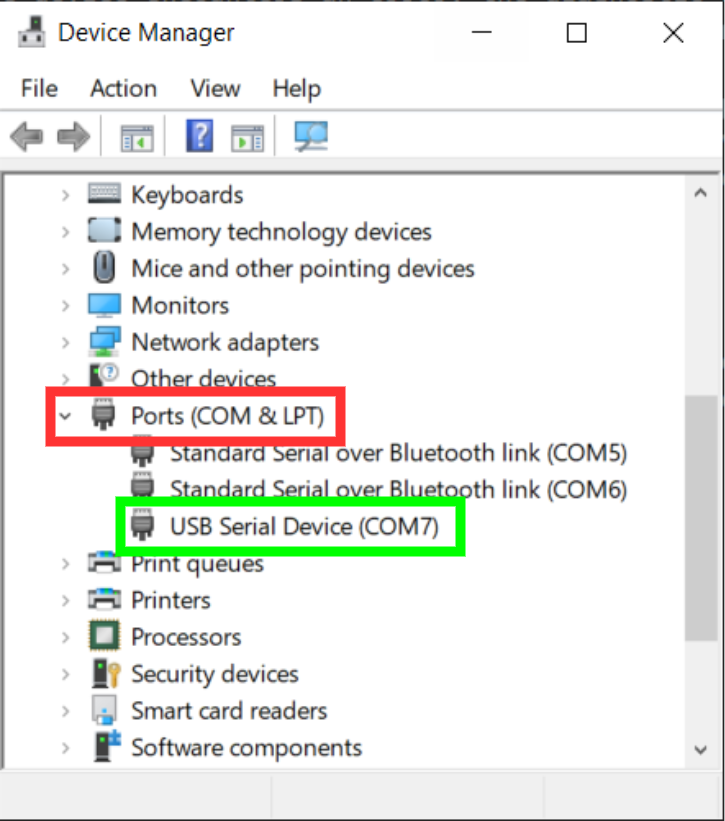
\includegraphics[width=0.45\textwidth]{troubleshooting/device_manager.png} \label{subfig:device_manager}} \hskip3ex
    \subfloat[In a serial terminal like PuTTy, enter the serial port from the device manager (green) and set the baudrate to 115200 (cyan)]{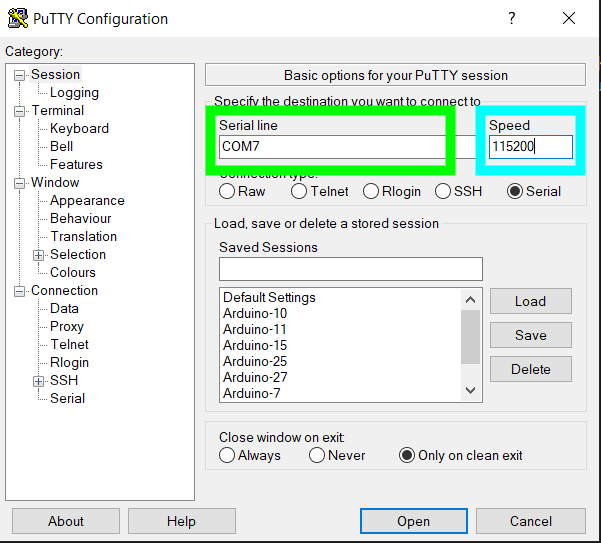
\includegraphics[width=0.45\textwidth]{troubleshooting/putty.png} \label{subfig:putty}}
    \caption{Opening the serial terminal for Thetis diagnostics}
    \label{fig:open_serial_terminal}
\end{figure}

Once the serial monitor is connected, there will be a string of data coming through.
At the start of the stream will be the diagnostic data from the initialization procedure.
The diagnostic messages are in the format: ``[Timestamp] [Log Level] Message'' where the timestamp is the current system time in ISO8601 format\footnote{yyyy-MM-ddThh:mm:ss.SSS}.
The log level is defined in \Fref{tab:log_level}.
By default, Thetis will report everything that is ``Verbose'' or below over the USB serial connection.

\customTable
{l c m{0.6\textwidth}}
{Level Name & Priority & Description}
{
    BYPASS & 0 & Indicates a message should just be passed along - only used for bypassing the typical log functions \\
    FATAL & 1 & Indicates a fatal event that cripples the device \\
    ERROR & 2 & Indicates a major error, but not fatal \\
    WARN & 3 & Indicates a substantial event that is not an error or fatal \\
    INFO & 4 & Indicates basic information for logging \\
    DEBUG & 5 & Indicates some parameter that is less important than basic information \\
    VERBOSE & 6 & Indicates some information that is less important than debug information \\
    TRACE & 7 & Information that can be used to trace down a specific bug or code execution sequence \\
}
{Log levels used by Thetis for diagnostics and their meanings}
{tab:log_level}

\begin{figure}[H]
    \centering
    \subfloat[If the device encounters an error on startup, the diagnostic log will report a ``FATAL'' event. Here, the microSD card is not present, so the filesystem fails to initialize]{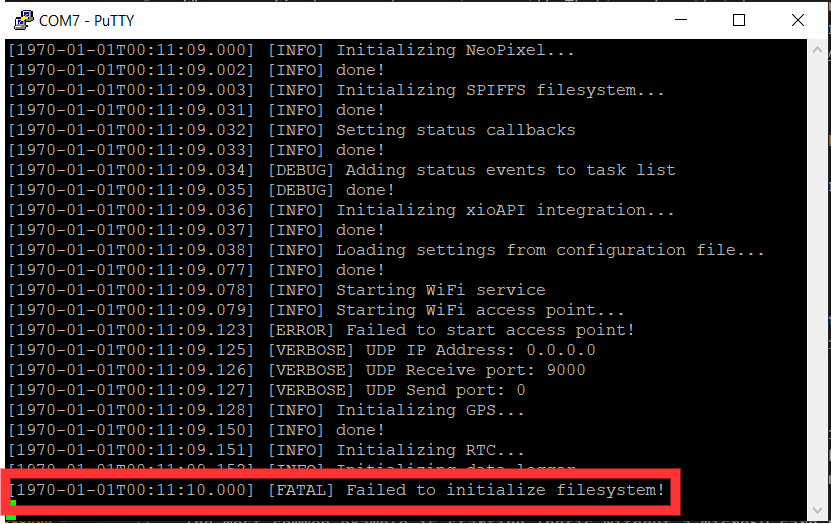
\includegraphics[width=0.45\textwidth]{troubleshooting/putty_output_error.png} \label{subfig:putty_output_error}} \hskip3ex
    \subfloat[When the device boots without error, there should be a long stream of data messages (green) after the initialization steps]{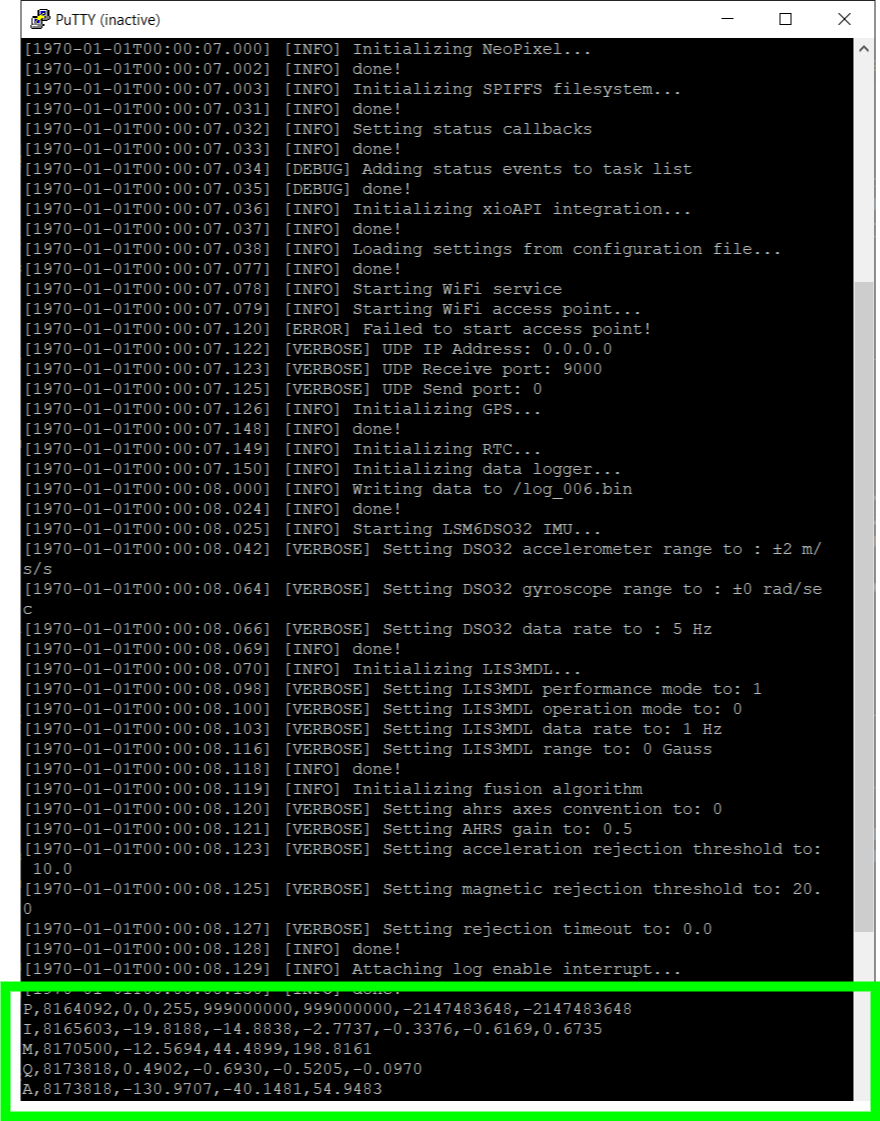
\includegraphics[width=0.45\textwidth]{troubleshooting/putty_output_good.png} \label{subfig:putty_output_good}}
    \caption{Different terminal outputs for Thetis based on error (left) or no error (right)}
    \label{fig:putty_outputs}
\end{figure}

\warning{If you are going to create a GitHub issue with your problem, it is \textbf{VERY RECOMMENDED} to include the diagnostic output from the serial monitor with your ticket. This will make diagnosing the problem easier.}

\subsection{Known Issues and Workarounds} \label{sec:known_issues}

\subsubsection{Diagnostic LED Not Working on Startup} 
When Thetis is first started, it will run through an initialization process to ensure all components are present and operating correctly.
During booting, if the device encounters an error, the diagnostic LED will not begin flashing.
The LED will remain off, but the GPS Fix and power LEDs will continue to illuminate as expected.

The most common example is starting Thetis without a microSD card present as shown in \Fref{fig:filesystem_error_bug}. 
The card is not present in the receptacle (red circle), but the device has booted without the RGB diagnostic LED illuminating any colors.
To fix this issue, place the microSD card in the receptacle and press the ``Reset'' button.
The device should start normally.

\begin{figure}[H]
    \centering
    \includegraphics[width=0.5\textwidth]{troubleshooting/filesystem_error_bug.png}
    \caption{The microSD card is not present at startup, but the device does not blink an error code.}
    \label{fig:filesystem_error_bug}
\end{figure}

\subsubsection{Thetis Not Showing Up in x-IMU3 GUI}
When Thetis is connected to a host computer over USB, it will not automatically start broadcasting data or interact with the x-IMU3 GUI.
This is because the firmware is in a diagnostic state and waiting for a serial terminal to open before streaming data.
Therefore, when using Thetis with the x-IMU3 GUI, plug it in, turn on the device and open a serial monitor to it as described above.
Then, open the x-IMU3 GUI and the device should be present.

\subsubsection{The Sensors are Reporting Data, but it is all Zeros}
Sometime